\documentclass[tikz,border=5pt]{standalone}
\usetikzlibrary{arrows.meta}
\begin{document}
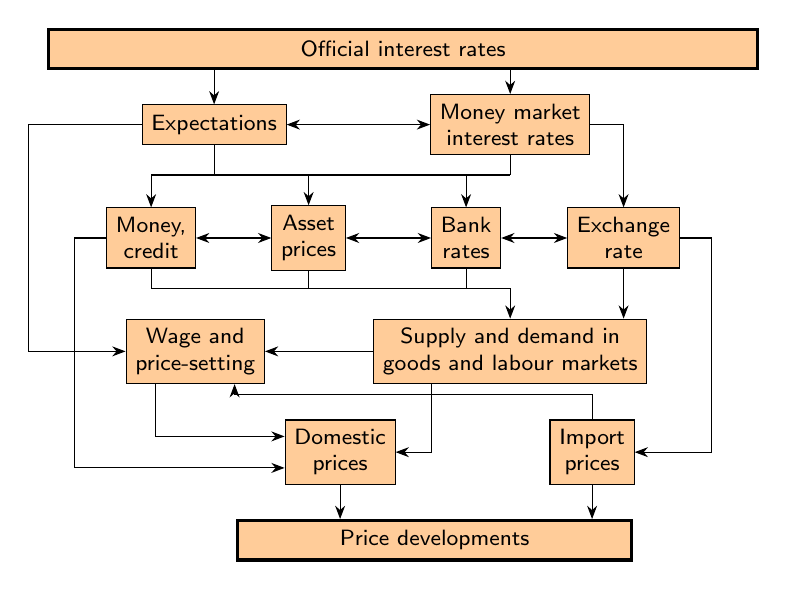
\begin{tikzpicture}[x=0.8cm,y=0.8cm,
  box/.style={draw, align=center, minimum height=5mm,fill=orange!40, font=\sffamily\footnotesize},
  >=Stealth]

% ecb_transmission

% --- Main boxes ---
\node[box, very thick, minimum width=9cm] (oir) at (-0.5,8) {Official interest rates};
\node[box] (exp)  at (-3.5,6.8) {Expectations};
\node[box] (mm)   at (1.2,6.8)  {Money market\\interest rates};
\node[box] (mon)  at (-4.5,5)   {Money,\\credit};
\node[box] (ast)  at (-2,5)     {Asset\\prices};
\node[box] (bnk)  at (0.5,5)    {Bank\\rates};
\node[box] (exr)  at (3,5)      {Exchange\\rate};
\node[box] (wage) at (-3.8,3.2) {Wage and\\price-setting};
\node[box] (sd)   at (1.2,3.2)  {Supply and demand in\\goods and labour markets};
\node[box] (dom)  at (-1.5,1.6) {Domestic\\prices};
\node[box] (imp)  at (2.5,1.6)  {Import\\prices};
\node[box, very thick, minimum width=5cm] (pd) at (0,0.2) {Price developments};

\coordinate (bus1) at (0,6);
\coordinate (bus2) at (0,4.2);

% --- Arrows ---
\draw[->] (exp |- oir.south) -- (exp);
\draw[->] (mm  |- oir.south) -- (mm);
\draw[<->] (exp) -- (mm);

\draw (exp.south) -- (exp.south |- bus1);
\draw (mm.south)  -- (mm.south |- bus1);
\draw (mon.north |- bus1) -- (mm.south |- bus1);
\foreach \n in {mon,ast,bnk} \draw[->] (\n.north |- bus1) -- (\n.north);
\draw[->] (mm) -| (exr);

\draw[<->] (mon) -- (ast);
\draw[<->] (ast) -- (bnk);
\draw[<->] (bnk) -- (exr);

\foreach \n in {mon,ast,bnk} \draw (\n.south) -- (\n.south |- bus2);
\draw (mon.south |- bus2) -- (sd.north |- bus2);
\draw[->] (sd.north |- bus2) -- (sd.north);
\draw[->] (exr.south) -- (exr.south |- sd.north);

\draw[->] (sd) -- (wage);
\draw[->] ([xshift=-1cm]sd.south) |- (dom.east);
\draw[->] ([xshift=-5mm]wage.south) |- ([yshift=2mm]dom.west);
\draw[->] (imp.north) -- ++(0,0.4) -| ([xshift=5mm]wage.south);
\draw[->] (exp.west) -- ++(-1.8,0) |- (wage.west);
\draw[->] (mon.west) -- ++(-0.5,0) |- ([yshift=-2mm]dom.west);
\draw[->] (exr.east) -- ++(0.5,0) |- (imp.east);
\draw[->] (dom) -- (dom |- pd.north);
\draw[->] (imp) -- (imp |- pd.north);

% % --- External shocks ---
% \draw[dashed] (5.2,0.2) coordinate (dash) -- (5.2,7.6);
% \node[box, text width=2.8cm, align=left] at (7.2,8.2)
%   {Shocks outside the control of the central bank};
% \foreach \t [count=\i] in {Changes in risk premia, Changes in bank capital,
%   Changes in the global economy, Changes in fiscal policy,
%   Changes in commodity prices} {
%   \node[box, text width=2.6cm, align=left] (s\i) at (7.2,8-1.3*\i) {\t};
%   \draw[->] (s\i.west) -- (s\i.west -| dash);
% }
\end{tikzpicture}
\end{document}